\documentclass[10pt]{book}
\usepackage{cdt/cdtBusiness}

%%%%%%%%%%%%%%%%%%%%%%%%%%%%%%%%%%%%%%%%%%%%%%%%%%%%%%%%%%%%%%%%
% Datos del proyecto

\cdtOrganizacion[CNSNS--SENER]{Comisión Nacional de Seguridad Nuclear y Salvaguardias, SENER}

\cdtAutor{Coordinación de Desarrollo Tecnológico, IPN}

\cdtSistema[REPO]{Subsistema de Repositorio de Información}

\cdtProyecto[234412, IPN-23.13-SCOR2]{Sistema de Control Radiológico Versión 2.0.}

\cdtDocumento{Propuesta}{Propuesta técnica}{\DRAFT{\today}} %\RELEASE{1.0}

\cdtEntregable{E1}{Entregable 1}

% Descomentar y establecer la fecha cuando se desee congelar la fecha del documento.
%\fecha{12 de Abril de 2013}

%%%%%%%%%%%%%%%%%%%%%%%%%%%%%%%%%%%%%%%%%%%%%%%%%%%%%%%%%%%%%%%%

\begin{document}

%=========================================================
% Portada
\thispagestyle{empty}

\maketitle

%=========================================================
% Indices del documento
\frontmatter
\tableofcontents
\listoffigures
\listoftables
\mainmatter

%=========================================================
\chapter{Modelo estructural del negocio}

	En esta sección se modelan las {\em Afirmaciones Estructurales del negocio} las cuales están conformadas por los {\em Términos del negocio} y los {\em Hechos del negocio}. Primero se especifica el {\em Contexto} en el que los términos tienen significado y las {\em Políticas del negocio} que modelan el presente modelo. 
	
	En las secciones \ref{sec:terminosDeNegocio} y \ref{sec:hechosDeNegocio} se presentan los Términos del negocio a manera de Glosario y por último se presentan los Hechos del negocio a manera de relaciones entre términos del negocio.

%----------------------------------------------------------
\section{Contexto}

	\cdtInstrucciones{El contexto debe explicar bajo que ambiente los términos del negocio son aplicables y proporcionar información general para su comprensión inicial.\\}
	La empresa ``Fast Rent'' se dedica a la renta de vehículos automotores, principalmente automóviles y motocicletas. Los clientes rentan vehículos por tiempos determinados y la empresa se encarga de dar mantenimiento a los vehículos y administrarlos para que estén disponibles para sus clientes. Los empleados, se dedican a labores de gerencia, atención a clientes, mantenimiento y soporte para los vehículos activos.

%----------------------------------------------------------
\section{Políticas}


%----------------------------------------------------------
\section{Términos del negocio}
\label{sec:terminosDeNegocio}

\begin{brGlosario}[version=1.0,]
	\brTermLiteral{tAutomovil}{Automóvil:}{tVehiculo}{Vehículo} De cuatro ruedas con capacidad de 5 a 9 personas. 
	\brTermType{tCliente}{Cliente:} Se refiere a todas las personas físicas y morales que \cdtRef{tRenta}{rentan} o han rentado un \cdtRef{tVehiculo}{vehículo}.
	
	\brTermLiteral{tDirector}{Director:}{tEmpleado}{Empleado} Es el empleado que tiene mayor rango de todos y no tiene superior, a diferencia de los demás.
	
	\brTermType{tEmpleado}{Empleado:} Se refiere a cualquier persona que labore en la empresa.
	
	\brTermClock{tChecador}{Checador:}{Hora de entrada y salida de un \cdtRef{tEmpleado}{empleado}.}{Una vez al día para la entrada y otra para la salida durante los días laborales.}
	
	\brTermLiteral{tMotocicleta}{Motocicleta:}{tVehiculo}{Vehículo} De dos ruedas con capacidad para una personas. 

	\brTermType{tRenta}{Renta:} Se refiere al servicio que ofrece la empresa para prestar \cdtRef{tVehiculo}{vehículos} a los \cdtRef{tCliente}{clientes} por un tiempo definido.
	
	\brTermType{tVehiculo}{Vehiculo:} Se refiere a los automóviles y motocicletas que la empresa usa para dar el servicio de renta a los \cdtRef{tCliente}{clientes}.
	
	\brTermSensor{tVelocimetro}{Velocímetro:}{Velocidad de un Vehículo.}{Kilometros/hora.}{Constantemente siempre que el \cdtRef{tVehiculo}{vehículo} esté encendido.}
\end{brGlosario}

%----------------------------------------------------------
\section{Hechos del negocio}
\label{sec:hechosDeNegocio}


%- - - - - - - - - - - - - - - - - - - - - - - - - - - - - 
\subsection{Modelo del dominio del problema}

\begin{figure}[htbp!]
	\begin{center}
		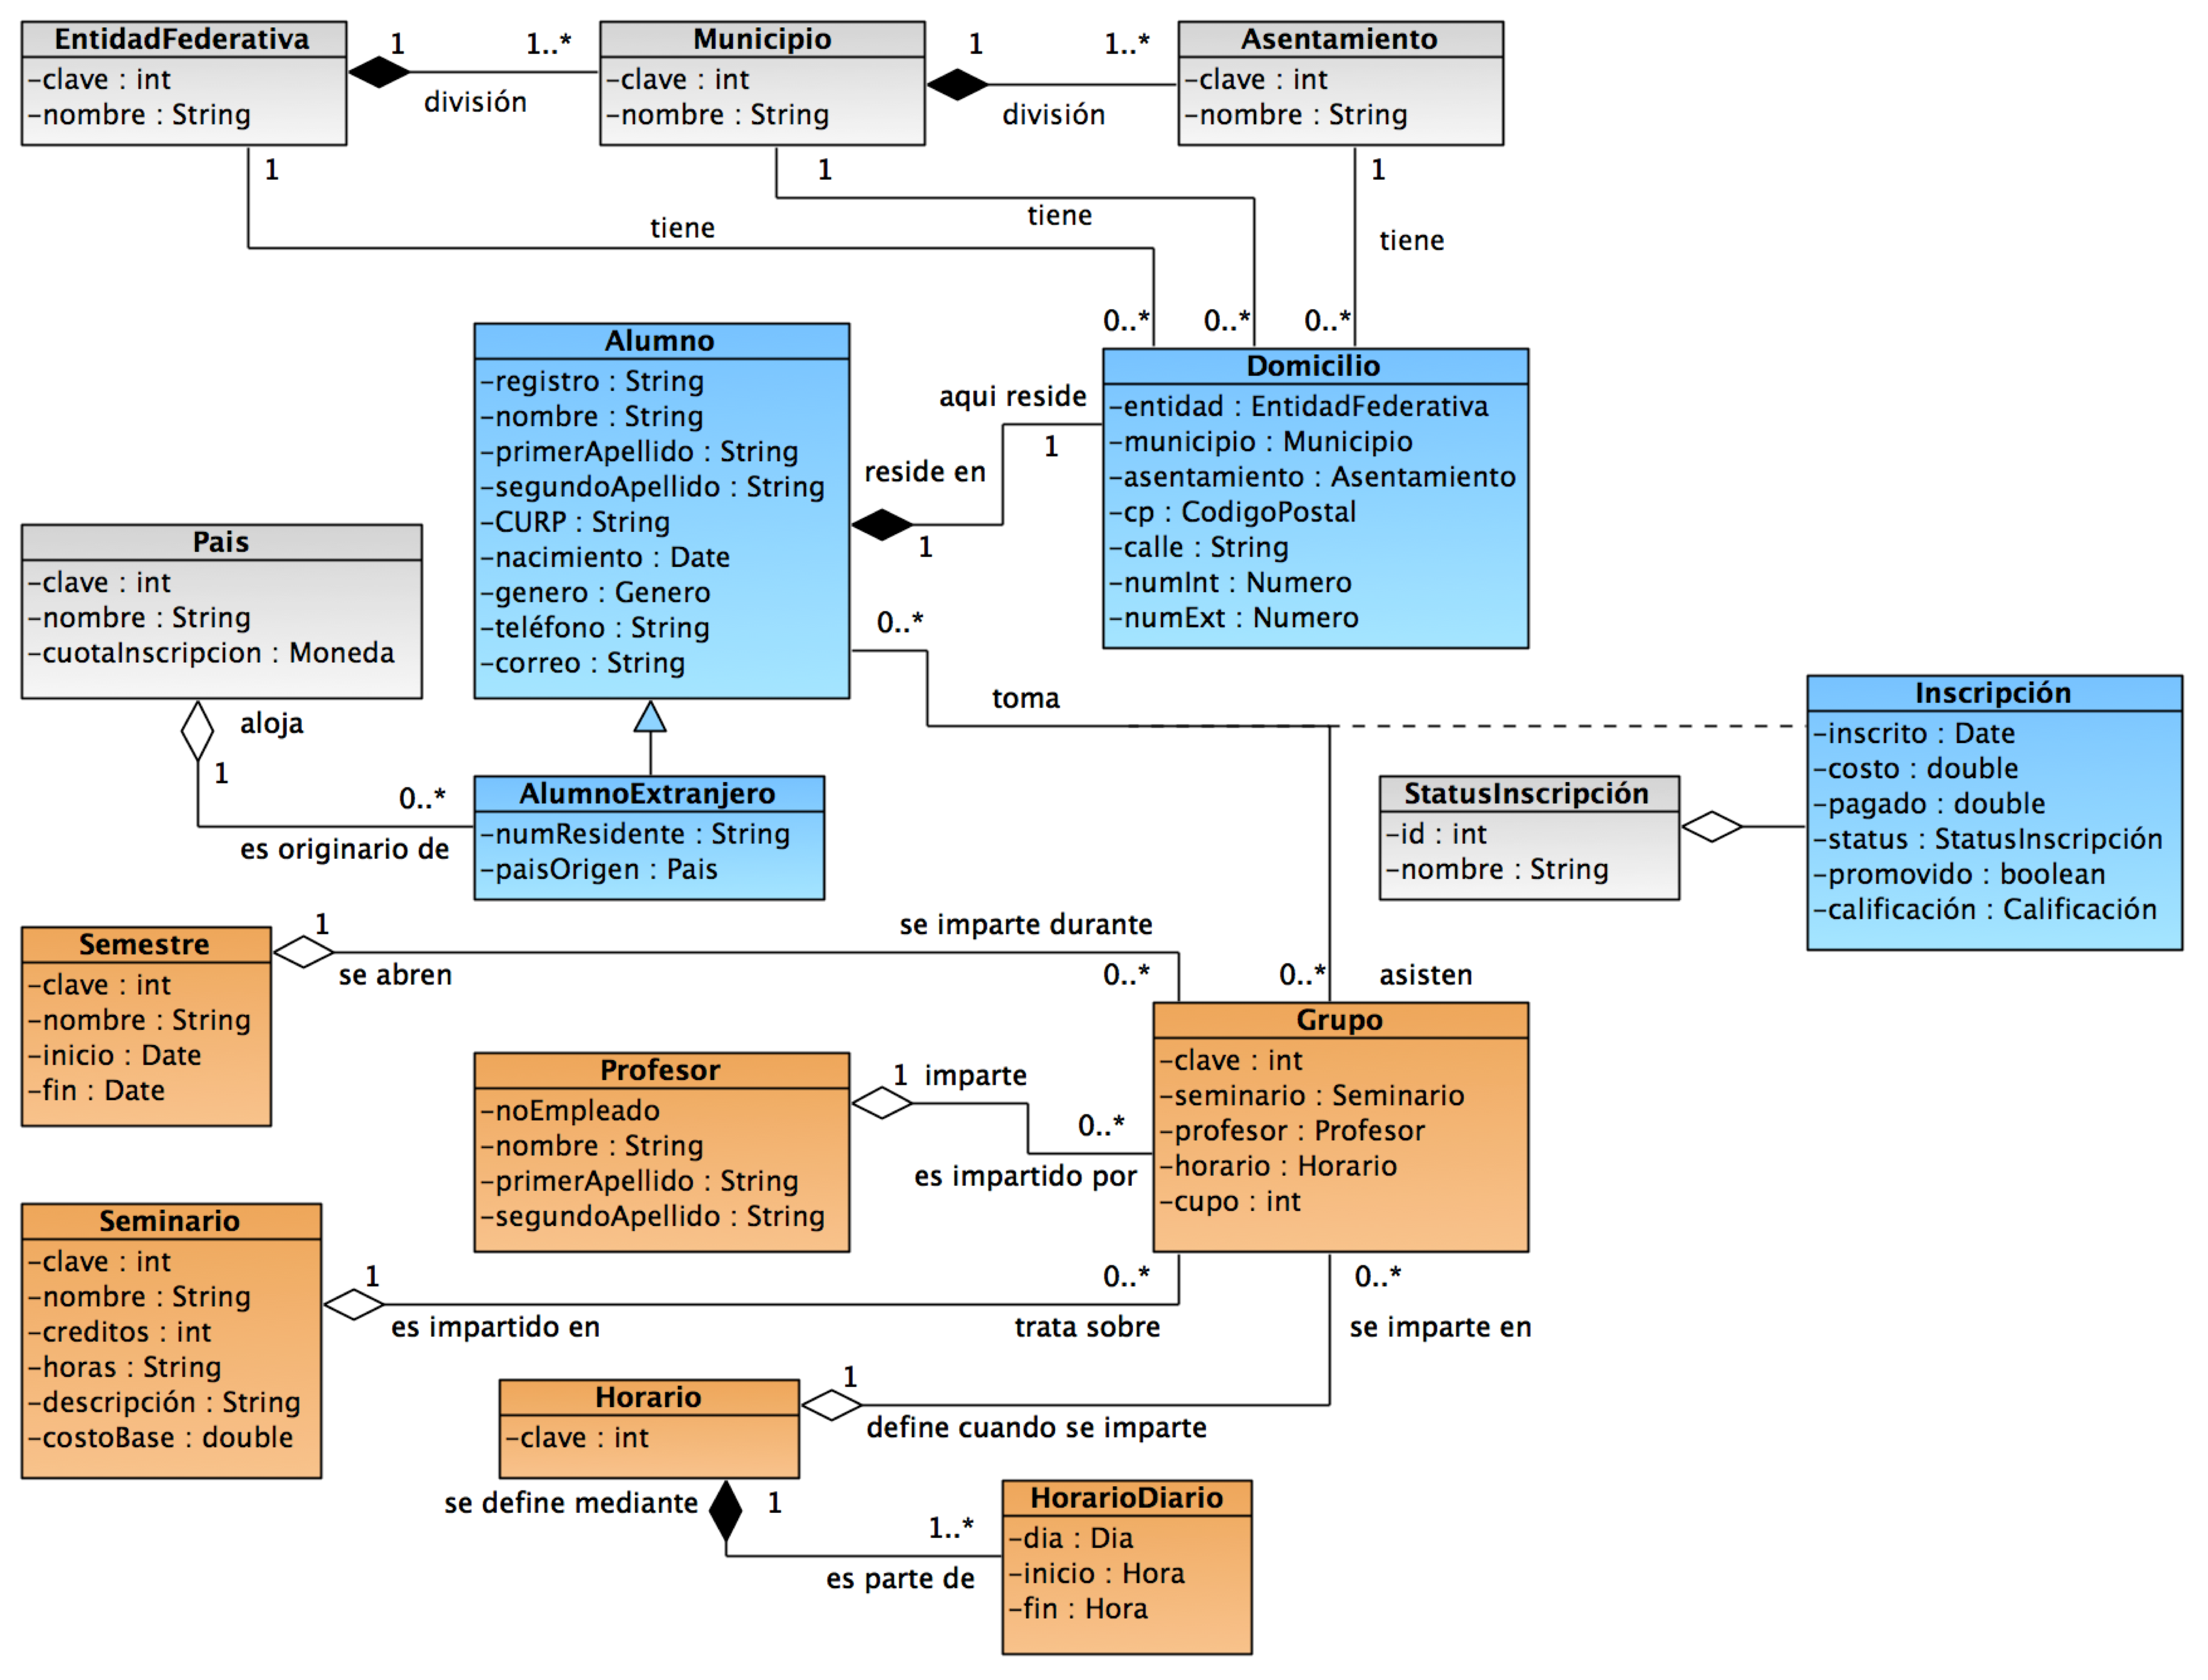
\includegraphics[angle=90,width=.95\textwidth]{images/modeloDelDominioDelProblema}
		\caption{Modelo del dominio del problema}
		\label{fig:modeloDeDominio}
	\end{center}
\end{figure}

%- - - - - - - - - - - - - - - - - - - - - - - - - - - - - 
\subsection{Tipos de datos base}

	Definición de los tipos de dato base base para el sistema.

\begin{description}
    \addDataType{dtId}{Id}{10 Dígitos.}
    	{10\dataType{Dígito}10}
	
    \addDataType{dtPalabraCorta}{Palabra corta}{Palabra de no más de 20 caracteres.}
    	{0\dataType{Caracter}20}
    
    \addDataType{dtPalabraLarga}{Palabra larga}{Palabra de no más de 50 caracteres.}
    	{0\dataType{Caracter}50}
    
    \addDataType{dtFrase}{Frase}{Frase larga de aproximadamente dos renglones.}
    	{0\dataType{Caracter}250}
    
    \addDataType{dtTexto}{Texto}{Texto de varios renglones.}
    	{0\dataType{Caracter}1500}
    
    \addDataType{dtCURP}{CURP}{Cédula Única de Registro de Población palabra de 18 caracteres.}
    	{4\dataType{Letra}4 + 6\dataType{Dígito}6 + \dataLiteral{'H' $|$ 'M'} + 5\dataType{Letra}5 + 2\dataType{Caracter}2}
    
    \addDataType{dtRFC}{RFC}{Registro Federal de Contribuyente}
    	{4\dataType{Letra}4 + 6\dataType{Dígito}6}
    
    \addDataType{dtRFCH}{RFC con homoclave}{Registro Federal de Contribuyente con homoclave.}
    	{4\dataType{Letra}4 + 6\dataType{Dígito}6 + 3\dataType{Caracter}3}
    
    \addDataType{dtTelefono}{Teléfono}{Número telefónico de 8 o 10 caracteres o con clave internacional.}
    	{\dataLiteral{ 
			{\color{black}8\dataType{Dígito}8} $|$
			{\color{black}10\dataType{Dígito}10} $|$
			'+'{\color{black} + 10\dataType{Dígito}11} 
		}}
    
    \addDataType{dtCorreo}{Correo}{Dirección de correo electrónico.}
    	{2\dataType{Caracter}50 + '{\tt @}' + 2\dataType{Caracter}50 + '{\tt.}' + 1\dataType{Letra}3} 

    \addDataType{dtNumeracion}{Numeración}{Número de un domicilio, puede ser: sin número, valor numérico y valor alfanumérico.}
    	{\dataLiteral{
			('S' + 'N') $|$
			1\dataType{Dígito}5 $|$
			1\dataType{Letra}5?
		}} 

    \addDataType{dtCantidadMonetaria}{Cantidad monetaria}{Se refiere a una cantidad de dinero.}
    	{'\$' + 1\dataType{Dígito}50 + '{\tt .}' + 2\dataType{Dígito}2} 

    \addDataType{dtGenero}{Género}{Genero masculino o femenino.}
    	{( \dataString{Masculino} $|$ \dataString{Femenino} )
		} 

    \addDataType{dtFecha}{Fecha}{Se refiere a un valor que especifica un día definido en el calendario.}
    	{2\dataType{Dígito}2 + '{\tt /}' + 2\dataType{Dígito}2 + '{\tt /}' + 4\dataType{Dígito}4} 

    \addDataType{dtHora}{Hora}{Se refiere a una hora especifica durante el día en formato de 24 hrs.}
    	{2\dataType{Dígito}2 + '{\tt :}' + 2\dataType{Dígito}2} 

    \addDataType{dtBooleano}{Booleano}{Valor Falso o Verdadero.}
    	{( \dataString{Verdadero} $|$  \dataString{Falso} )}

    \addDataType{dtDia}{Día}{Se refiere a un día de la semana.}
    	{( \dataString{Lunes} $|$ \dataString{Martes} $|$ \dataString{Miércoles} $|$ 
			\dataString{Jueves} $|$ \dataString{Viernes} $|$ \dataString{Sábado} $|$\\
			\dataString{Domingo} )}

    \addDataType{dtCalificacion}{Calificación}{Es la calificación que obtiene un alumno.}
    	{ \dataLiteral{'A' $|$ 'B' $|$ 'C' $|$ 'D' $|$ 'E' $|$ 'F'} + \dataLiteral{ '' $|$ '-' $|$ '+' $|$ '++'} }
	
    \addDataType{dtCodigoPostal}{Código postal}{Es el código dado por el servicio postal a un asentamiento.}
    	{ 5\dataType{Dígito}5 } 

\end{description}

%- - - - - - - - - - - - - - - - - - - - - - - - - - - - - 
\subsection{Tipos de datos compuestos}

\begin{brCombinedType}{dtEntidadFederativa}{Entidad Federativa}
	\brAttr{clave}{Clave}{dtId}
		{clave de la Entidad federativa, dada por INEGI}{Sí}
	\brAttr{nombre}{Nombre}{dtPalabraCorta}
		{Nombre oficial de la Entidad federativa dado por INEGI}{Sí}
\end{brCombinedType}

%\begin{brCombinedType}{dtNombreTipoCompuesto}{nombreTipoCompuesto}{
%		% Estados: \ccEdicion, \ccTerminado, \ccRevisado, \ccAprobado, 
%		\begin{techCard}{Version}{Nombre del Autor}{Estado}
%			\tItem{Revisor}{Nombre del revisor}
%		\end{techCard}
%	}
%	\brAttr{idAttr}{nombreAttr}{tipoAttr}
%		{descripcionAttr}{opcional: sí/no}
%	\brEntityRelSection
%	% tipos de relacion: \brRelComposition, \brRelAgregation, \brRelGeneralization
%	\brRel{tipoDeRelacion}{Entidad destino}{Un \refElem{Alumno} reside en un \refElem{Domicilio}}	

\begin{brCombinedType}{dtDomicilio}{Domicilio}
	\brAttr{entidadFederativa}{Entidad federativa}{dtEntidadFederativa}
		{Entidad del domicilio}{Sí}
	\brAttr{municipio}{Municipio}{dtMunicipio}
		{Municipio del domicilio}{Sí}
	\brAttr{asentamiento}{Asentamiento}{dtAsentamiento}
		{Colonia, barrio, unidad, etc. del domicilio}{No} 
	\brAttr{calle}{Calle}{dtPalabraLarga}
		{Calle sobre la cual se encuentra el domicilio}{Sí}
	\brAttr{cp}{Código Postal}{dtCorreo}
		{Uno de los códigos postales dados por el servicio postal al asentamiento del domicilio.}{No} 
	\brAttr{numExterior}{Número exterior}{dtNumeracion}
		{Segundo apellido del cliente}{No} 
	\brAttr{numInterior}{Número interior}{dtNumeracion}
		{Segundo apellido del cliente}{No} 
\end{brCombinedType}

%- - - - - - - - - - - - - - - - - - - - - - - - - - - - - 
\begin{brEntity}{Alumno}{Alumno}
	\brAttr{registro}{Registro}{dtId}{Número de registro utilizado para identificar un alumno}{Si}
	\brAttr{nombre}{Nombre}{dtPalabraCorta}
		{Nombre o nombres del alumno.}{Sí}
	\brAttr{primerApellido}{Primer apellido}{dtPalabraCorta}
		{Primer apellido del alumno.}{Sí}
	\brAttr{segundoApellido}{Segundo apellido}{dtPalabraCorta}
		{Segundo apellido del alumno.}{No}
	\brAttr{CURP}{CURP}{dtCURP}
		{CURP del alumno.}{Sí}
	\brAttr{nacimiento}{Nacimiento}{dtFecha}
		{Fecha de nacimiento del alumno.}{Sí}
	\brAttr{genero}{Género}{dtDomicilio}
		{Género del alumno.}{No}
	\brAttr{telefono}{Teléfono}{dtTelefono}
		{Teléfono para contactar al alumno.}{Sí}
	\brAttr{correo}{Correo}{dtCorreo}
		{Correo del alumno para enviar información académica y escolar y para recuperación de clave de acceso.}{Sí}
	\brEntityRelSection
	\brRel{\brRelComposition}{Domicilio}{Un \refElem{Alumno} reside en un \cdtRef{Domicilio}{Domicilio}}	
	\brRel{\brRelAgregation}{Grupo}{Un \cdtRef{Alumno}{Alumno} toma un \cdtRef{Curso}{Curso}}	
\end{brEntity}

%- - - - - - - - - - - - - - - - - - - - - - - - - - - - - 
\cdtSetKey{author=Ulises Vélez Saldaña, version=1.0}
\begin{brEntity}{AlumnoExtranjero}{Alumno Extranjero}%{}
	\brAttr{numeroResidente}{Numero de residente}{dtId}{Número de registro dado por la Secretaría de Relaciones Exteriores a los extranjeros.}{Si}
	\brAttr{paisOrigen}{Pais origen}{Pais}
		{País de origen del alumno extranjero.}{Sí}
	\brEntityRelSection
	\brRel{\brRelAgregation}{País}{Un \cdtRef{Alumno}{Alumno} es originario de un \cdtRef{Pais}{Pais}}	
	\brRel{\brRelGeneralization}{Alumno}{Un \cdtRef{AlumnoExtranjero}{Alumno Extranjero} es un  \cdtRef{Alumno}{Alumno}}	
\end{brEntity}


%- - - - - - - - - - - - - - - - - - - - - - - - - - - - - 

\begin{brEntity}[author=Juan, version=1.1]{Alumno2}{Alumno 2}%{}
	\brAttr{numeroResidente}{Numero de residente}{dtId}{Número de registro dado por la Secretaría de Relaciones Exteriores a los extranjeros.}{Si}
	\brAttr{paisOrigen}{Pais origen}{Pais}
		{País de origen del alumno extranjero.}{Sí}
	\brEntityRelSection
	\brRel{\brRelAgregation}{País}{Un \cdtRef{Alumno}{Alumno} es originario de un \cdtRef{Pais}{Pais}}	
	\brRel{\brRelGeneralization}{Alumno}{Un \cdtRef{AlumnoExtranjero}{Alumno Extranjero} es un  \cdtRef{Alumno}{Alumno}}	
\end{brEntity}
ñlkasdfklj aslkf klasdjhfkjasdf lkjasdhflkjasdhf lkajs dflkjasdhflkjasdhf lkjdsflkj,ahsdfl kjad s f l k jdfslkj adsflkjd sflkjad sflkj adsl kfjh als kdj, fha sdfkjhasdlkjfh alskd flkasdjf lkajsdhf lkajsd flkjasdhflkasd
%- - - - - - - - - - - - - - - - - - - - - - - - - - - - - 
\begin{brEntity}{Alumno3}{Alumno 3}%{}
	\brAttr{numeroResidente}{Numero de residente}{dtId}{Número de registro dado por la Secretaría de Relaciones Exteriores a los extranjeros.}{Si}
	\brAttr{paisOrigen}{Pais origen}{Pais}
		{País de origen del alumno extranjero.}{Sí}
	\brEntityRelSection
	\brRel{\brRelAgregation}{País}{Un \cdtRef{Alumno}{Alumno} es originario de un \cdtRef{Pais}{Pais}}	
	\brRel{\brRelGeneralization}{Alumno}{Un \cdtRef{AlumnoExtranjero}{Alumno Extranjero} es un  \cdtRef{Alumno}{Alumno}}	
\end{brEntity}

\section{Reglas de negocio}

\begin{bRule}[author=Juan, version=1.1]{BR8}{Fecha de Nacimiento correcta}
	{\brtIntegrity}% Otras opciones: \brtOperation, \brtInference
	{\brcAssertion}% Otras opciones: \brcTimed, \brcEjecutive
	{\brnControl}% Otras opciones: \brnInfluence
    %- - - - - - - - - - - - - - - - - - - - - - - - - - - - - - 
	\brItem{Descripción}{
	Las Fechas de Nacimiento que se registran en el SINACEM para cualquier Persona debe ser mayores al día Primero de Enero del año 1900 y menor a la Fecha Actual.}
	\brItem{Motivación}{Evitar fraudes al PRONIM por el registro de personas que no han nacido al momento de su registro.}
	\brItem{Sentencia}{$\forall p \in Persona \Rightarrow 01-Enero-1900~<~p.fechaDeNacimiento~<~fechaActual$}
	\brItem[brCompilanceColor]{Ejemplo positivo}{Para el día 12 de Octubre del 2013, cumplen la regla: 		
        \begin{Citemize}
        	\item 11 de Octubre del 2013
			\item 20 de Diciembre del 2010
			\item 2 de Enero del 1900
        \end{Citemize}
	}
	\brItem[brNotCompilanceColor]{Ejemplo negativo}{Para el día 12 de Octubre del 2013, no cumplen la 
		\begin{Citemize}
        	\item 12 de Octubre del 2013
			\item 20 de Diciembre del 2014
			\item 1 de Enero del 1900
			\item 31 de Diciembre del 1899
        \end{Citemize}
	}
	\brItem{Referenciado por}{\cdtRef{CUCE3.2}{CUCE3.2}, \cdtRef{CUCE3.3}{CUCE3.3}}
\end{bRule}

\begin{bRule}{BR8}{Fecha de Nacimiento correcta}
	{\brtIntegrity}% Otras opciones: \brtOperation, \brtInference
	{\brcAssertion}% Otras opciones: \brcTimed, \brcEjecutive
	{\brnControl}% Otras opciones: \brnInfluence
	\brItem{Descripción}{
	Las Fechas de Nacimiento que se registran en el SINACEM para cualquier Persona debe ser mayores al día Primero de Enero del año 1900 y menor a la Fecha Actual.}
	\brItem{Motivación}{Evitar fraudes al PRONIM por el registro de personas que no han nacido al momento de su registro.}
	\brItem{Sentencia}{$\forall p \in Persona \Rightarrow 01-Enero-1900~<~p.fechaDeNacimiento~<~fechaActual$}
	\brItem[brCompilanceColor]{Ejemplo positivo}{Para el día 12 de Octubre del 2013, cumplen la regla: 		
        \begin{Citemize}
        	\item 11 de Octubre del 2013
			\item 20 de Diciembre del 2010
			\item 2 de Enero del 1900
        \end{Citemize}
	}
	\brItem[brNotCompilanceColor]{Ejemplo negativo}{Para el día 12 de Octubre del 2013, no cumplen la 
		\begin{Citemize}
        	\item 12 de Octubre del 2013
			\item 20 de Diciembre del 2014
			\item 1 de Enero del 1900
			\item 31 de Diciembre del 1899
        \end{Citemize}
	}
	\brItem{Referenciado por}{\cdtRef{CUCE3.2}{CUCE3.2}, \cdtRef{CUCE3.3}{CUCE3.3}}
\end{bRule}

%==========================================================
\clossing
\end{document}
